\documentclass[a4paper]{article}
%\usepackage[utf8]{inputenc}
\usepackage[english]{babel}
\usepackage[T1]{fontenc}

\setlength{\parindent}{0pt}
\setlength{\parskip}{2ex}

%\usepackage[backend=biber, style=apa]{biblatex}
%\usepackage{csquotes}
%\addbibresource{sources.bib}

\usepackage{mathtools}

\usepackage{graphicx}

\usepackage{amsthm} 

\usepackage{amsfonts} 

\usepackage{amssymb}

\usepackage{txfonts}

\usepackage{microtype}

\usepackage{setspace}

\usepackage{hyperref}

\usepackage{hyphsubst}

\usepackage{float}

\usepackage{enumitem}


\hypersetup{hidelinks}

\usepackage{geometry}
\usepackage{setspace}
\geometry{a4paper,left=60pt,right=60pt,top=60pt, bottom=60pt}
\spacing{1.2}

\makeatletter
\renewcommand*\env@matrix[1][*\c@MaxMatrixCols c]{%
  \hskip -\arraycolsep
  \let\@ifnextchar\new@ifnextchar
  \array{#1}}
\makeatother

\theoremstyle{definition}
\newtheorem{theorem}{Theorem}[section]
\theoremstyle{definition}
\newtheorem{sats}[theorem]{Sats}
\theoremstyle{definition}
\newtheorem{example}[theorem]{Example}
\theoremstyle{definition}
\newtheorem{exempel}[theorem]{Exempel}
\theoremstyle{definition}
\newtheorem{definition}[theorem]{Definition}
\theoremstyle{definition}
\newtheorem{corollary}[theorem]{Corollary}
\theoremstyle{definition}
\newtheorem{korollarium}[theorem]{Korollarium}
\theoremstyle{definition}
\newtheorem{lemma}[theorem]{Lemma}
% \theoremstyle{definition}
% \newtheorem{proof}[theorem]{Proof}
\theoremstyle{definition}
\newtheorem{bevis}[theorem]{Bevis}
\theoremstyle{definition}
\newtheorem{metod}[theorem]{Metod}
\theoremstyle{definition}
\newtheorem{method}[theorem]{Method}
\theoremstyle{definition}
\newtheorem{problem}[theorem]{Problem}
\theoremstyle{plain}
\newtheorem{obs}[theorem]{OBS!}

\newcommand{\opim}{\operatorname{im}}
\newcommand{\opker}{\operatorname{ker}}
\newcommand{\opspan}{\operatorname{span}}
\newcommand{\opmean}[1]{\overline{#1}}
\newcommand{\opconj}[1]{\overline{#1}}
 


\title{Bayesian Inference}
\author{William Kraft}
\date{Farum Math Camp 2024}

\begin{document}

\maketitle
\tableofcontents
\subsection{What is probability?}

\begin{definition}[Outcome]
	An outcome is a possible result form an experiment. They are mutually exclusive, and contain all relevant data about the result.
\end{definition}

\begin{definition}[Sample Space]
	The sample space, denoted \(\Omega\), of an experiment is the set of all possible outcomes.
\end{definition}

\begin{definition}[Event]
	An event is a subset of the sample space. We say it occurs if the outcome is an element in the event.
\end{definition}

\begin{definition}~
	\begin{itemize}
		\item The complementary event, \(A^*\) of \(A\) is the complement of \(A\)
		\item The union of the events \(A\) and \(B\) is the set \(A \cup B\) 
		\item The intersection of the events \(A\) and \(B\) is the set \(A \cap B\) 
		\item The events \(A\) and \(B\) are mutually exclusive if they are disjoint, \(A \cap B = \emptyset\) 
	\end{itemize}
\end{definition}

\begin{obs}
	The terms from probability theory will be used interchangeably with their set theoretic counterparts.
\end{obs}

\begin{definition}[Probability measure]
	A probability measure \(P( \cdot )\) is a function from an event to a real number which follows ``Kolmogorov's System of Axioms'':
	\begin{enumerate}[leftmargin = 3em, wide=1em, label={Axiom \arabic*:}]
		\item If \(A\) is any event, then \(0 \leq P(A) \leq 1\) 
		\item If \(\Omega \) is the entire sample space, then \(P(\Omega ) = 1\) 
		\item If \(A\), \(B\), \(\dots \)  is a finite or infinite sequence of mutually exclusive events, then \(P(A \cup B \dots) = P(A) + P(B) + \dots  \)
	\end{enumerate}
	There are often multiple reasonable probability measures, but this allows us to easily work with any of them.
\end{definition}

\begin{example}[Frequency probability measure]
	Given a repeatable experiment we define the frequency probability measure is the relative frequency of the event.
\end{example}

\begin{example}[Other probability measure]
	Often probability measures can be subjective. For example, what was the probability of a soccer match ending the way it did? We can not recreate it exactly, and so there is no way to use the frequency probability measure. Instead it would depend on who you asked. As long as their probability concurs with Kolmogorov's axioms, we can work with it! 
\end{example}

\begin{corollary}[Basic Rules]
	From the axioms it can be proven that
	\begin{itemize}
		\item \(P(A^*) = 1 - P(A)\) 
		\item \(P(\emptyset ) = 0\)
		\item \(P(A) + P(B) = P(A \cup B) - P(A \cap B)\) 
	\end{itemize}
\end{corollary}

\begin{definition}[Discrete and continuous sample space]
	If a sample space is either finite or countably infinite it is discrete. Otherwise, it is continuous.
\end{definition}

\begin{example}
	The different outcomes of a 6 sided dice are discrete while its exact landing spot is continuous. Note that the same experiment may have different sample spaces depending on what you are studying.
\end{example}


\newpage
\section{Probability Theory}
\subsection{Motivation}
The world is full of systems where no model we can construct, either due to complexity or lack of data, could produce accurate results. Probability theory instead attempts to find patterns within the chaos, making us able to still study these random, stochastic, systems.


\subsection{Conditional Probability}


\begin{definition}[Conditional probability]
	The probability of \(A\) \textbf{given} (an outcome of) \(B\) is defined as
	\[
		P(A|B) = \frac{P(A \cap B)}{P(B)}.
	\]
\end{definition}

\begin{obs}
	This definition of conditional probability is quite natural as it preserves relative probability, and gives the new sample space probability 1.
\end{obs}

\begin{obs}
	The probability measure \(P( \cdot | B)\) also satisfies Kolmogorov's axioms.
\end{obs}

\begin{example}
	The probability of having rolled a 5 on a 6 sided die \textbf{given} that the result was odd, is \(\frac{1}{3}\).
\end{example}

\begin{theorem}[Total Probability Theorem]
	Let \(B_1, \dots, B_n\) be mutually exclusive events and their union be the sample space. If \(A\) is an event, then
	\[
		P(A) = P(\cup _{k=1} ^{n} A \cap B_k) = \sum_{k=1}^{n} P(A \cap B _k) =  \sum_{k=1}^{n} P(A|B_k)  \cdot P(B_k)
	\]
\end{theorem}


\begin{theorem}[Bayes' Theorem]
	Let \(A_1, \dots, A_n\) be mutually exclusive events and their union be the sample space. If \(B\) is an event, then
	\[
		P(A_i|B) = \frac{P(B|A_i) \cdot P(A_i)}{P(B)} = \frac{P(B|A_i) \cdot P(A_i)}{\sum_{k=1}^{n} P(B|A_k)  \cdot P(A_k)}  
	\]
\end{theorem}

\begin{definition}[Independent events]
	The events \(A\) and \(B\) are independent, \(A \perp B\),  if
	\[
		P(A \cap B) = P(A)P(B).
	\]
\end{definition}

\begin{obs}
	This does not imply, for example, that they are independent given C.
\end{obs}

\subsection{Random variables}

\begin{definition}[Random variables]
	A random variable (rv) is a function from our sample space to \(\mathbb{R}\) .
\end{definition}

\begin{example}
	Consider the experiment of throwing a dart at a dartboard. Let \(X\) be the number of centimeters from the bullseye. Then \(X\) is a random variable. We could have many random variables stemming from the same experiment.
\end{example}

\begin{example}
	Let \(X\) be the price of a match (in £), and \(Y\) be the price of a can of gasoline. Then the cost of both is \(X + Y\). If \(Z\) is the number of times you do this purchase, the total cost is \((X+Y) \cdot Z\).
\end{example}

\begin{obs}
	We often write the shorthand of \(P(\text{condition} )\) to denote \(P(A)\) where \(A\) is the set of all outcomes satisfying the condition. For example \(P(X = 1)\) where \(X\) is the result of a 6-sided die.
\end{obs}

\begin{definition}[Outcome of a random variable]
	An outcome of a random variable is a value obtained by running the experiment. Multiple outcomes of a known random variable are independent.
\end{definition}

\begin{example}
	Let \(X\) be the number of leafs on a clover when you pick it up. If i pick up a lucky clover (4 leafs), it means the outcome of picking that clover was \(x = 4\).
\end{example}

\subsection{Distributions}
\begin{definition}
	The distribution function (cumulative distribution function) of a random variable \(X\) is defined as
	\[
		F_X(x) = P(X \leq x).
	\]
	Note that \(X\) is the random variable, while \(x\) is an argument to the function. 
\end{definition}

\begin{corollary}
	A distribution function \(F_X(x)\) of a random variable \(X\) has that
	\begin{align}
		&F_X(X) \rightarrow \begin{cases} 0 \\ 1 \end{cases} \text{ when } x \rightarrow \begin{cases} - \infty \\ \infty  \end{cases}  \\
		&F_X(x) \text{ is a non-decreasing function of } x \\
		&F_X(x) \text{ is continuous from the right for any} x
	\end{align}
\end{corollary}

\begin{theorem}
	\[
		P(a < X \leq b) = F_X(b) - F_X(a)
	\]
\end{theorem}


\begin{definition}[Probability function]
	For a discrete random variable \(X\) (from a discrete sample space), the probability function is
	\[
		f_X(x) = P(X = x)
	\]
\end{definition}

\begin{theorem}
	The sum
	\[
		\sum_{x = -\infty }^{\infty} f_X(x) = 1
	\]
\end{theorem}

\begin{definition}[Density function]
	Let \(X\) be a continuous random variable. If the distribution function can be written as
	\[
		F_X(x) = \int_{- \infty } ^x f_x(t)dt,
	\]
	then \(f_X(x)\) is called the density function (probability density function), and \(X\) is a continuous random variable.
\end{definition}

\begin{obs}
	We will often be able to work similarly with continuous and discrete random variables, with the only mayor difference being integration vs summation. As we will focus more on continuous functions in the following lectures, I might exclude the discrete case at times.
\end{obs}



\begin{definition}[Distribution]
	A distribution function corresponds to a unique distribution. Two stochastic variables have the same distribution, if they have the same distribution functions.
\end{definition}

\begin{obs}
	This gives us a way to look at the properties of categorising random variables without looking at their corresponding sample spaces.
\end{obs}

\begin{example}
	A continuous random variable \(X\) has a uniform distribution on the interval \((a, b)\) (written \(X \sim U(a, b)\)) if
	\[
		F_X(x) = \begin{cases} 0, x < a \\ 1, x > b \\ \frac{x-a}{b-a}, \text{ otherwise}   \end{cases} 
	\]
\end{example}

\begin{obs}
	Both the probability function and density function, also uniquely correspond to a distribution function. We may even say it has the distribution of such a function.
\end{obs}

\begin{example}
	A discrete random variable \(X \sim \operatorname{Bin} (n, p)\) if
	\[
		f _X (x)= \binom{n}{x} p ^{x} (1-p) ^{n-x},
	\]
	where \(0 \leq x \leq n \).
	
\end{example}



% TODO!!! Perhaps avoid these?

\begin{theorem} % TODO Double check
	Let \(X, Y\) be discrete random variables with \(Y= g(X)\) and \(g\) invertible. Then
	\[
		f_Y(y) = P(Y = y) = P(g(X) = y) = P(X = g^{-1}(y))=f_X(g^{-1}(y))
	\]
	If \(g\) is not invertible, then
	\[
		f_Y(y) = P(Y = y) =P(g(X) = y) = \sum_{x \in A} P(X = x)=\sum_{x \in A}f_X(x)
	\]
	where \(A = \left\{x | g(x) = y\right\}\).

\end{theorem}

\begin{theorem}
	Let \(X, Y\) be random variables with \(Y= g(X)\) and \(g\) strictly increasing. Then
	\[
		F_Y(y) = P(Y \leq y) = P(g(X) \leq y) = P(X \leq g^{-1}(y)) = F_X(g^{-1}(y))
	\]
	If \(g\) strictly decreasing
	\[
		F_Y(y) = P(Y \leq y) = P(g(X) \leq y) = P(X \geq g^{-1}(y)) = 1 - F_X(g^{-1}(y)).
	\]
\end{theorem}


\begin{theorem}
	Let \(X, Y\) be continuous random variables with \(Y= g(X)\), \(g\) continuous and bijective. Then 
	\[
		f_Y(y) = F_Y'(y) = \begin{cases} F_X'(g^{-1}(y)) \cdot g^{-1} ~'(y) \\ -F_X'(g^{-1}(y)) \cdot g^{-1} ~'(y) \end{cases} = f_X(g^{-1}(y)) \cdot g^{-1} ~'(y).
	\]
\end{theorem}

\subsection{Multivariate distributions}
\begin{obs}
	We may without problem choose two or more random variables from a single experiment.
\end{obs}

\begin{definition}
	Given the random variables \(X_1, \dots , X_n\), we can define:
	\begin{itemize}
		\item The distribution function
			\[
				F_{X_1, \dots , X_n}(x_1, \dots , x_n) = P(X_1 \leq x_1 \land \dots \land X_n \leq x_n).
			\]
		\item The probability function (given \(X_i\) discrete)
			\[
				f_{X_1, \dots , X_n}(x_1, \dots , x_n) = P(x_1, \dots, x_n).
			\]
		\item The density function, \(f\) which satisfies: (given \(X_i\) continuous)
			\[
				\underset{\mathbb{R} \times \dots \times \mathbb{R}}{\int \cdots \int} F _{X_1, \dots, X_n}(x_1, \dots ,x_n) (x_1, \dots, x_n) dx_1 \dots dx_n.
			\]
	\end{itemize}
\end{definition}


\begin{theorem} % Double check this. Possibly add a special case for 2 variables
	Let \(\vec{X}, \vec{Y}\) be vectors of random variables with \(\vec{Y} = g(\vec{X})\) and \(g\) bijective, continuous. Then
	\[
		f_Y(y) = f_X(g^{-1}(y))  \cdot |\det J| 
	\]
	where \(J\) is the Jacobian of \(g^{-1}\). (Proven using variable substitution for integrals)
\end{theorem}

\begin{definition}[Marginal distribution]
	Let \(X, Y\) be two random variables with the distribution function \(F _{X, Y}(X,Y)\). Then the marginal distribution of \(X\) is
	\[
		F_X(x) = \lim_{y \rightarrow \infty } F_{X, Y}(x, y).
	\]
	With a similar spirit, we can define the marginal probability function as
	\[
		f_X(x) = \sum_{y = - \infty } ^{\infty } P _{X, Y}(x, y)
	\]
	and the marginal density function
	\[
		f_X(x) = \int_{-\infty }^{\infty} f _{X, Y}(x,y) dy.
	\]
\end{definition}

\begin{example}
	Let \(X, Y\) be the results of two 6-sided dice. As they are independent, the probability function would be
	\[
		f _{X, Y}(x, y) = f _X(x)  \cdot f_Y (x) = \frac{1}{6}  \cdot \frac{1}{6} = \frac{1}{36}
	\]
	where \(1 \leq X, Y \leq 6\).
	The marginal distribution of \(X\) would be
	\[
		f _{X}(x) = \sum_{y=1}^{6} f _{X, Y} (x, y) = \frac{1}{6} 
	\]
	
\end{example}

\begin{definition}[Distribution given]
	The density function of \(X | Y\) is
	\[
		f _{X|Y}(x|y) = \frac{f _{X, Y}(x, Y)}{f _{Y}(y)}.
	\]
	where \(f _{Y}(y)\) is the marginal density function of \(f _{X, Y}(x, y)\).
\end{definition}

\begin{example}
	Let \(X, Y\) be result of two independent dice, and \(Z = X+Y\). When given the result of \(X\), we have 
	\[
		f _{Z| X}(z| x) = f _{Y}(z-x).
	\]
\end{example}


\subsection{Exercise Problems}

\begin{problem}
	The probability of having a certain disease is \(0.01\), the probability of getting a positive test result is \(0.9\) if you have the disease, and \(0.01\) if you dont. Given a positive test result, what is the probability of you having the disease?
\end{problem}

\begin{problem}
	Let \(X\) be a continuous variable which is uniformly distributed on \((a, b)\). What is the distribution of \(Y = \frac{X}{2} + 3\)?
\end{problem}

\begin{problem}
	What is the probability function of the sum of one 6-sided die and one 8-sided die?
\end{problem}

\begin{problem} % TODO CHECK
	You want to burn up a few documents in your backyard. The time in minutes, \(T\), it takes for all documents to have been burnt up is distributed as \(T \sim Exp(r)\) where \(R\) is the burn rate of the gasoline you choose. As your time is limited, the chance of you choosing the fast burning new gasoline with burn rate \(10\) is \(30\%\) and otherwise you choose the old with burn rate \(2\). What is the chance of you having burnt everything within 5 minutes?
\end{problem}

\begin{problem}
	A friend picked randomly between a 4, 6, and 8 sided die and only told you they rolled a 3. What is the probability they rolled the 4-sided die? If they roll again with the same die, what is the probability they roll a 5?
\end{problem}

\begin{problem}
	Given the distribution of \(X|\Theta\) and \(\Theta\), what is the distribution of \(X\)? What is the distribution of \(\Theta |X\)?
\end{problem}

\newpage
\section{Bayesian Inference}
\subsection{Situations} % Change title
Using probability theory, we can calculate the chances of events given the distribution. While the type of distribution can often be inferred, finding the hidden parameter is a very challenging task.


\subsection{Philosophy}
Bayesian inference is based around the idea that one never encounters a situation without previous knowledge! For example, you may know, that the dice is likely fair, and otherwise, probably loaded in favor of higher numbers. This information is as valuable as any other, and should be combined with your new observations. Using this, we can calculate the chances of you rolling quintuple sixes... \textbf{given} your previous knowledge, and the fact you have already rolled quadruple sixes. This is achieved by not considering the probabilities as constants, but as random variables themselves.

\subsection{Prior distribution}
\begin{definition}
	Let \(X\) be a random variable with a distribution depending on the outcome \(\theta \) of the random variable \(\Theta \). The distribution of \(\Theta \) is called the \textit{prior} distribution, while the distribution of \(X|\Theta \) is called the data distribution.

	The prior distribution represents your prior knowledge of the parameter, while the data distribution represents the distribution of \(X\) given you know the outcome of \(\Theta \) which the distribution depends on. 
\end{definition}

\begin{example}
	Let the result of a coin flip (0 if tails, 1 if heads) be \(X|\Theta \sim \operatorname{Ber}(\theta )\) where \(\theta\) is the chance of flipping heads. When seeing a new coin its properties affect the chances of flipping heads, and might be distributed as \(\Theta \sim \operatorname{Beta}(2, 2)\). The former is the data distribution, the latter the prior distribution.
\end{example}

\begin{obs}
	Most further calculations will be done only in the continuous case, the discrete case is left as an exercise.
\end{obs}


\begin{definition}[Prior predictive distribution]
	The distribution of \(X\) is the called the prior predictive distribution. It is what we, before observing more data, would find to be the distribution of \(X\). It is calculated from our prior distribution and data distribution, as the marginal distribution of the simultaneous distribution 
	\[
		f_{X, \Theta }(x,\theta) = f_\Theta(\theta )  \cdot f _{X|\Theta }(x|\theta ).
	\]
	That is,
	\[
		f_X(x) = \int_{-\infty }^{\infty} f_\Theta(\theta )  \cdot f _{X|\Theta }(x|\theta ) d \theta 
	\]
	
\end{definition}


\subsection{Posterior distribution}
The goal of Bayesian inference is creating the posterior distribution \(\Theta | X=x \) where \(x \) is an outcome of the random variable \(X\). That is, using the previous outcomes, we update our belief of what the distribution of \(\Theta \) may be.

\begin{definition}[Posterior distribution] % Adjust to allow for more outcomes
	The posterior distribution \(\Theta |x\) is defined as
	\[
		f _{\Theta |X}(\theta |x) = \frac{f _{X|\Theta}(x|\theta )  \cdot f_\Theta (\theta )}{f_X(x)} 
	\]
	and is simply an application of Bayes' rule!!!
\end{definition}

\begin{obs}
	Once we have calculated the posterior distribution, we may calculate anything we would ever want to know about the distribution of \(X\).
\end{obs}

\begin{obs}
	The gamma function is defined as 
	\[
		\Gamma(x) = \int_{0}^{\infty} t^{x-1} \cdot e^{-t}dt
	\]
	and has the property \(\Gamma(x)  \cdot x = \Gamma(x+1)\) 
\end{obs}


\begin{example}
	Let \(\Theta \sim \operatorname{Gamma}(\alpha , \lambda)\) (the prior distribution) and \(X \sim \operatorname{Exp}(\theta) \) (the data distribution). The density functions become
	\begin{align*}
		f _{\Theta}(\theta) &= \frac{\lambda ^ \alpha }{\Gamma (\alpha )} \theta ^{\alpha -1} e ^{-\lambda \theta } \\
		f _{X | \Theta }(x | \theta ) &= \theta e ^{-\theta x}
	\end{align*}
	where \(\theta , x > 0\).

	The prior predictive distribution becomes
	\begin{align*}
		f _{X }(x) &= \int_{0}^{\infty} f _{x, \Theta }(x, \theta) d \theta \\
							 &= \int_{0}^{\infty} f _{\Theta }(\theta ) f _{X | \Theta }(x | \Theta ) d \theta \\
							 &= \int_{0}^{\infty} \frac{\lambda ^ \alpha }{\Gamma (\alpha )} \theta ^{\alpha -1} e ^{-\lambda \theta }  \cdot \theta e ^{-\theta x} \\
							 & = \frac{\lambda ^ \alpha }{\Gamma (\alpha )} \int_{0}^{\infty} \theta ^{\alpha } e ^{- \theta (x + \lambda )}d \theta \\ 
							 & = \frac{\lambda ^ \alpha }{\Gamma (\alpha )} (\lambda +x ) ^{- \alpha -1} \int_{0}^{\infty} u ^{\alpha } e ^{- u}du \\
							 & = \frac{\lambda ^ \alpha }{\Gamma (\alpha )} (\lambda +x ) ^{- \alpha -1} \Gamma(\alpha+1) \\
							 & = \alpha \lambda ^ \alpha  (\lambda +x ) ^{- \alpha -1}
	\end{align*}

	We may then calculate the posterior distribution
	\begin{align*}
		f _{\Theta |X}(x | \theta ) &= \frac{ f _{x, \Theta }(x, \theta) }{f _X (x)} \\
																&= \frac{f _{\Theta }(\theta ) f _{X | \Theta }(x | \Theta ) }{f _{X}(x)}  \\
																&= \frac{\frac{\lambda ^ \alpha }{\Gamma (\alpha )} \theta ^{\alpha -1} e ^{-\lambda \theta }  \cdot \theta e ^{-\theta x}}{\alpha \lambda ^ \alpha  (\lambda +x ) ^{- \alpha -1}} \\
																&= \frac{(\lambda + x)^{\alpha +1}}{\Gamma(\alpha ) \alpha } \theta ^{\alpha} e ^{\theta (\lambda +x)}\\
																&= \frac{(\lambda + x)^{\alpha +1}}{\Gamma(\alpha +1)} \theta ^{\alpha + 1 -1} e ^{\theta (\lambda +x)}
	\end{align*}
	Which we can easily recognise as the gamma distribution, giving us
	\[
		\Theta | X \sim \operatorname{Gamma}(\alpha +1, \lambda + x)  
	\]

	
\end{example}

\begin{definition}[Proportionality]
	A function \(f(x)\) is proportional to a function \(g(x)\) if there is a constant \(c \ne 0\) such that for all \(x\), 
	\[
		f(x) = c  \cdot g(x).
	\]

	We write this relationship
	\[
		f(x) \propto g(x).
	\]
	If they are dependent on multiple variables, the relevant one will be given by the context.
\end{definition}


\begin{example}
	Let \(\Theta \sim \operatorname{Beta} (\alpha , \beta )\) and \(X|\Theta \sim \operatorname{Bin}(n, \theta)\). The density functions will then be
	\begin{align*}
		f_ \Theta (\theta ) &= \frac{\Gamma(\alpha + \beta) }{\Gamma(\alpha )\Gamma(\beta )} \theta ^{\alpha -1} \theta ^{\beta -1} \\
		f _{X | \Theta }(x | \theta ) &= \binom{n}{x} \theta ^x (1-\theta ) ^{n-x} \\
	\end{align*}
	We notice that in respect to \(\theta \) the posterior distribution is proportional to
	\begin{align*}
		f _{\Theta |X}(\theta | x) 
			&= \frac{ f _{x, \Theta }(x, \theta) }{f _X (x)} \\
			&= f _{x, \Theta }(x, \theta) \\
			&= f _{x| \Theta }(x| \theta)  \cdot f _{\Theta } (\theta )\\
			&\propto \theta ^x (1-\theta ) ^{n-x}  \cdot \theta ^{\alpha -1} \theta ^{\beta -1} \\
			&= \theta ^{\alpha + x - 1} (1 - \theta ) ^{\beta + n - x - 1}. \\
	\end{align*}
	We notice that this is proportional to the beta distribution. As the integral of the function is 1, we can then scale the function to satisfy the criterion. We may otherwise notice this is a scaled version of the Beta distribution and scale it to match, giving us
	\[
		\Theta |X \sim \operatorname{Beta} (\alpha +x, \beta + n -x).
	\]
\end{example}


\begin{obs}
	Notice that this rule may be used to update the distribution multiple times. These updating rules can often be found in formula sheets, but are derived as above.
\end{obs}

\begin{example}
	Let \(\Theta \sim \operatorname{Beta} (2, 2)\) and \(X|\Theta \sim Ber(\theta)\). For example \(X\) could be \(1\) if we flip heads, and \(1\) if we flip heads. While flipping 5 heads in a row, and updating each time, we notice our distribution gets heavily skewed towards higher probabilities of heads.
	\begin{figure}[H]
		\centering
		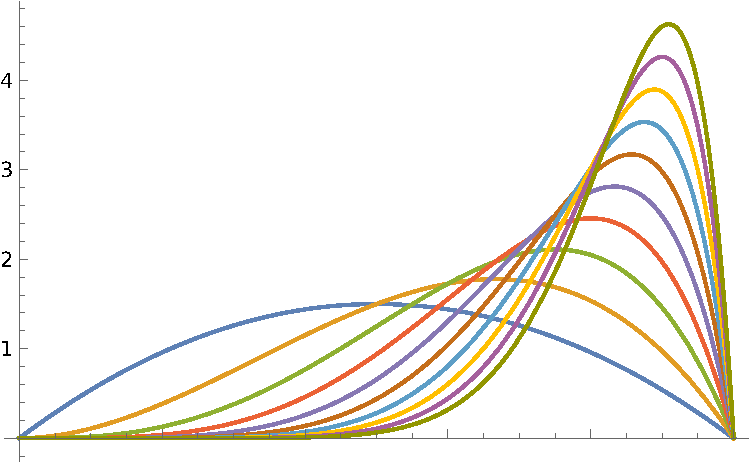
\includegraphics[width=0.5\textwidth]{beta.pdf}
	\end{figure}
	If our prior distribution had been less varied, the results would have been showing later.
\end{example}

\subsection{Exercise problems}

\begin{problem}
	Find the updating rule for \(X | \Theta  \sim \operatorname{Po} (\theta)\) and \(\Theta \sim \operatorname{Gamma} (\alpha, \lambda )\) where
	\[
		f _{X|\Theta }(x|\theta ) = \frac{e ^{- \lambda} \lambda ^x}{x!}.
	\]
\end{problem}

\begin{problem}
	Find the updating rule for \(\Theta \sim N(\mu , \sigma _1^2)\) and \(X | \Theta \sim N(\theta , \sigma _2^2 \) where the \(N(\mu , \sigma \) is the normal distribution with density function
	\[
		\frac{1}{\sqrt{2 \pi \sigma ^2} } e ^{- \frac{(x-\mu) }{2 \sigma ^2} }.
	\]
	Find the updating rule!
\end{problem}

\begin{problem}
	Given the posterior distribution, how would you find an interval where \(\Theta \) has \(p\) probability to be within it?
\end{problem}

\begin{problem}
	If you have the posterior distribution, and the data distribution. How could you calculate the posterior predictive distribution?
\end{problem}

\newpage
\section{Applications}
By now, we know the distribution of the parameter, and may calculate anything we want to know about the parameter or the distribution!

\subsection{Posterior predictive distribution}
\begin{definition}[Posterior predictive distribution]
	Let \(Y\) be a random variable which is identically distributed to \(X\). Given the prior distribution, data distribution and outcomes of \(X\), we may then calculate the simultaneous distribution of \(Y\) and \(\Theta \), and marginalise it to get the distribution of \(Y\). The latter is called the posterior predictive distribution and is (in the continuous case) calculated as
	\[
		f _{Y|X}(x|\theta ) = \int_{-\infty }^{\infty} f _{\Theta |X}(\theta|x )  \cdot f _{Y|\Theta }(y|\theta ) d \theta.
	\]
\end{definition}

\begin{obs}
	The posterior predictive distribution is very similar to the prior predictive distribution, but instead of using the prior distribution, it uses the posterior distribution.
\end{obs}

\subsection{Credibility interval}


\begin{definition}[Credibility interval]
	A credibility interval of \(\Theta\) is an interval \(I\) such that \(P(X \in I) = p\). 
\end{definition}

\begin{obs}
	We often choose a symmetric credibility interval, where \(X\) is equally likely to be lower or higher than the interval, but may choose it as we please as long as the probability of \(X\) falling within it is \(p\).
\end{obs}

\begin{obs}
	Quite often numerical approximation of integrals is used to find credibility intervals.
\end{obs}

\subsection{Decisions}
\begin{definition}[Expected Value]
	The expected value of function \(g\) of a continuous random variable \(X\) is 
	\[
		E\left[g(X)\right] = \int_{-\infty }^{\infty} g(x) f _{X}(x) dx.
	\]
\end{definition}

\begin{obs}
	The expected value is linear.
\end{obs}


\begin{definition}[Loss Function]
	The loss function
	\[
		L\left[\theta , a\right]
	\]
	where is a possible value of \(\Theta \), and \(a\) is an action, is the ``loss'' which occurs if we take the action \(a\) when \(\Theta \) has the value \(\theta \).
\end{definition}

\begin{definition}[Bayes Risk]
	The Bayes risk,
	\[
		E\left[L(\Theta, W(X))\right],
	\]
	is the expected loss when using the decisions rule \(W(x)\) to decide your action given observation
\end{definition}

\begin{theorem}[Minimising Bayes Risk]
	In order to minimise the Bayes risk however, notice that the outcome of \(X\) is already determined, and thus we simply minimize
	\[
		E\left[L(\Theta, W(x))| X\right] = \int_{- \infty }^{\infty} L(\theta , W(x))  \cdot f _{\Theta | X}(\theta |x) d \theta.
	\]
\end{theorem}

\begin{example}
	Let the action to be taken be, giving an estimate \(a\) of \(\theta\), and the loss function be \((\theta -a)^2\). We wish to minimize
	\[
		E[L(\Theta, a)|X] = E [ (\Theta - a)^2 |X] = E[\Theta ^2|X] -2aE[\Theta |X] + a^2.
	\]
	As we can only affect \(a\), we wish to minimize
	\[
		a^2-2aE[\Theta |X]
	\]
	which is done by setting \(a = E[\Theta |X]\).
\end{example}

\subsection{Bayesian Hierarchy}

\begin{definition}
	If \(X|\Theta \), \(\Theta | \Phi \) and \(\Phi \) have known distributions, we call this a Bayesian Hierarchy, where \(\Phi \) is a super parameter.
\end{definition}

\begin{example}
	Let \(X\) be the result of a chess player during a single match, \(\Theta \) be their ability depending on that day, and \(\Phi \) be their skill. Then by seeing results from matches, we can update our belief of their ability that day, and in turn, update our belief of their skill.
\end{example}

\subsection{Easier calculations}
While Bayesian inference gives a good framework for statistics, it also requires a lot of integrals. All the given examples have been nice in this regard, but one easily encounters situation where the integrals are unfeasible, or even unsolvable. In these cases we may leave them, and when calculating the final values simply approximate them. There are however some methods to make our lives easier.






\begin{definition}[Conjugating distributions]
	We call a prior distribution and a data distribution conjugating, if the posterior distribution is in the same family (of the same form) as the prior distribution.
\end{definition}

\begin{obs}
	These are often the nicest cases, and if within reason, we prefer to choose these types of distributions.
\end{obs}


\subsection{Exercise Problems}
\begin{problem}
	What would be the posterior distribution of \(\Phi \) in the example about a Bayesian Hierarchy?
\end{problem}


\begin{problem}
	Let \(X| \alpha , \beta \), what would be a conjugating distribution of \(\alpha, \beta \)? 
\end{problem}



%\printbibliography[heading=bibintoc,title=References,]
\end{document}
